\documentclass{article}

\usepackage{arxiv}

\usepackage[utf8]{inputenc} % allow utf-8 input
\usepackage[T1]{fontenc}    % use 8-bit T1 fonts
\usepackage{lmodern}        % https://github.com/rstudio/rticles/issues/343
\usepackage{hyperref}       % hyperlinks
\usepackage{url}            % simple URL typesetting
\usepackage{booktabs}       % professional-quality tables
\usepackage{amsfonts}       % blackboard math symbols
\usepackage{nicefrac}       % compact symbols for 1/2, etc.
\usepackage{microtype}      % microtypography
\usepackage{graphicx}

\title{Explaining time series downsampling through visualisation}

\author{
    Morgan Frodsham
   \\
    School of Computing \\
    Newcastle University \\
  Newcastle upon Tyne, UK \\
  \texttt{\href{mailto:M.C.M.Frodsham2@newcastle.ac.uk}{\nolinkurl{M.C.M.Frodsham2@newcastle.ac.uk}}} \\
   \And
    Matthew Forshaw
   \\
    School of Computing \\
    Newcastle University \\
  Newcastle upon Tyne, UK \\
  \texttt{\href{mailto:matthew.forshaw@newcastle.ac.uk}{\nolinkurl{matthew.forshaw@newcastle.ac.uk}}} \\
  }

% Pandoc syntax highlighting
\usepackage{color}
\usepackage{fancyvrb}
\newcommand{\VerbBar}{|}
\newcommand{\VERB}{\Verb[commandchars=\\\{\}]}
\DefineVerbatimEnvironment{Highlighting}{Verbatim}{commandchars=\\\{\}}
% Add ',fontsize=\small' for more characters per line
\usepackage{framed}
\definecolor{shadecolor}{RGB}{248,248,248}
\newenvironment{Shaded}{\begin{snugshade}}{\end{snugshade}}
\newcommand{\AlertTok}[1]{\textcolor[rgb]{0.94,0.16,0.16}{#1}}
\newcommand{\AnnotationTok}[1]{\textcolor[rgb]{0.56,0.35,0.01}{\textbf{\textit{#1}}}}
\newcommand{\AttributeTok}[1]{\textcolor[rgb]{0.77,0.63,0.00}{#1}}
\newcommand{\BaseNTok}[1]{\textcolor[rgb]{0.00,0.00,0.81}{#1}}
\newcommand{\BuiltInTok}[1]{#1}
\newcommand{\CharTok}[1]{\textcolor[rgb]{0.31,0.60,0.02}{#1}}
\newcommand{\CommentTok}[1]{\textcolor[rgb]{0.56,0.35,0.01}{\textit{#1}}}
\newcommand{\CommentVarTok}[1]{\textcolor[rgb]{0.56,0.35,0.01}{\textbf{\textit{#1}}}}
\newcommand{\ConstantTok}[1]{\textcolor[rgb]{0.00,0.00,0.00}{#1}}
\newcommand{\ControlFlowTok}[1]{\textcolor[rgb]{0.13,0.29,0.53}{\textbf{#1}}}
\newcommand{\DataTypeTok}[1]{\textcolor[rgb]{0.13,0.29,0.53}{#1}}
\newcommand{\DecValTok}[1]{\textcolor[rgb]{0.00,0.00,0.81}{#1}}
\newcommand{\DocumentationTok}[1]{\textcolor[rgb]{0.56,0.35,0.01}{\textbf{\textit{#1}}}}
\newcommand{\ErrorTok}[1]{\textcolor[rgb]{0.64,0.00,0.00}{\textbf{#1}}}
\newcommand{\ExtensionTok}[1]{#1}
\newcommand{\FloatTok}[1]{\textcolor[rgb]{0.00,0.00,0.81}{#1}}
\newcommand{\FunctionTok}[1]{\textcolor[rgb]{0.00,0.00,0.00}{#1}}
\newcommand{\ImportTok}[1]{#1}
\newcommand{\InformationTok}[1]{\textcolor[rgb]{0.56,0.35,0.01}{\textbf{\textit{#1}}}}
\newcommand{\KeywordTok}[1]{\textcolor[rgb]{0.13,0.29,0.53}{\textbf{#1}}}
\newcommand{\NormalTok}[1]{#1}
\newcommand{\OperatorTok}[1]{\textcolor[rgb]{0.81,0.36,0.00}{\textbf{#1}}}
\newcommand{\OtherTok}[1]{\textcolor[rgb]{0.56,0.35,0.01}{#1}}
\newcommand{\PreprocessorTok}[1]{\textcolor[rgb]{0.56,0.35,0.01}{\textit{#1}}}
\newcommand{\RegionMarkerTok}[1]{#1}
\newcommand{\SpecialCharTok}[1]{\textcolor[rgb]{0.00,0.00,0.00}{#1}}
\newcommand{\SpecialStringTok}[1]{\textcolor[rgb]{0.31,0.60,0.02}{#1}}
\newcommand{\StringTok}[1]{\textcolor[rgb]{0.31,0.60,0.02}{#1}}
\newcommand{\VariableTok}[1]{\textcolor[rgb]{0.00,0.00,0.00}{#1}}
\newcommand{\VerbatimStringTok}[1]{\textcolor[rgb]{0.31,0.60,0.02}{#1}}
\newcommand{\WarningTok}[1]{\textcolor[rgb]{0.56,0.35,0.01}{\textbf{\textit{#1}}}}

% tightlist command for lists without linebreak
\providecommand{\tightlist}{%
  \setlength{\itemsep}{0pt}\setlength{\parskip}{0pt}}

% From pandoc table feature
\usepackage{longtable,booktabs,array}
\usepackage{calc} % for calculating minipage widths
% Correct order of tables after \paragraph or \subparagraph
\usepackage{etoolbox}
\makeatletter
\patchcmd\longtable{\par}{\if@noskipsec\mbox{}\fi\par}{}{}
\makeatother
% Allow footnotes in longtable head/foot
\IfFileExists{footnotehyper.sty}{\usepackage{footnotehyper}}{\usepackage{footnote}}
\makesavenoteenv{longtable}

% Pandoc citation processing
\newlength{\cslhangindent}
\setlength{\cslhangindent}{1.5em}
\newlength{\csllabelwidth}
\setlength{\csllabelwidth}{3em}
\newlength{\cslentryspacingunit} % times entry-spacing
\setlength{\cslentryspacingunit}{\parskip}
% for Pandoc 2.8 to 2.10.1
\newenvironment{cslreferences}%
  {}%
  {\par}
% For Pandoc 2.11+
\newenvironment{CSLReferences}[2] % #1 hanging-ident, #2 entry spacing
 {% don't indent paragraphs
  \setlength{\parindent}{0pt}
  % turn on hanging indent if param 1 is 1
  \ifodd #1
  \let\oldpar\par
  \def\par{\hangindent=\cslhangindent\oldpar}
  \fi
  % set entry spacing
  \setlength{\parskip}{#2\cslentryspacingunit}
 }%
 {}
\usepackage{calc}
\newcommand{\CSLBlock}[1]{#1\hfill\break}
\newcommand{\CSLLeftMargin}[1]{\parbox[t]{\csllabelwidth}{#1}}
\newcommand{\CSLRightInline}[1]{\parbox[t]{\linewidth - \csllabelwidth}{#1}\break}
\newcommand{\CSLIndent}[1]{\hspace{\cslhangindent}#1}

\begin{document}
\maketitle


\begin{abstract}
Enter the text of your abstract here.
\end{abstract}

\keywords{
    blah
   \and
    blee
   \and
    bloo
   \and
    these are optional and can be removed
  }

\twocolumn

\hypertarget{introduction}{%
\section{INTRODUCTION}\label{introduction}}

The UK Government is committed to making data-driven decisions that
engender public trust
\protect\hyperlink{ref-data2017}{{[}1{]}}--\protect\hyperlink{ref-data2022}{{[}4{]}}.
Data-driven decisions are considered to be ``more well-informed''
\protect\hyperlink{ref-data2017}{{[}1{]}}, effective
\protect\hyperlink{ref-data2022}{{[}4{]}}, consistent
\protect\hyperlink{ref-data2021}{{[}3{]}}, and better ``at scale''
\protect\hyperlink{ref-data2020}{{[}2{]}}. Despite this, there is a lack
of trust in government use of data
\protect\hyperlink{ref-trust}{{[}5{]}}. This suggests that public trust
in data-driven decisions goes beyond how the ``data complies with legal,
regulatory and ethical obligations''
\protect\hyperlink{ref-data2021}{{[}3{]}}. Transparency is needed for
the UK public to have ``confidence and trust in how data, including
personal data, is used'' \protect\hyperlink{ref-data2020}{{[}2{]}},
\protect\hyperlink{ref-trust}{{[}5{]}}.

To make data-driven decisions, government decision-makers also need to
trust the data and how it is used. This means trusting which data points
are selected, how this data collected and stored, and the capability of
data practitioners to understand the quality, insights and limitations
of it. At every stage of the data processing pipeline, data
practitioners have the opportunity to communicate the impact of the
assumptions and choices they are making to support decision-makers in
trusting the data informing their decisions.

Time series data is used across the UK Government
\protect\hyperlink{ref-pathway}{{[}6{]}} to inform for decision-makers
across various domains \protect\hyperlink{ref-onstool}{{[}7{]}}. The
volume of time series data has been increasingly continuously
\protect\hyperlink{ref-datapoint}{{[}8{]}}, posing significant
challenges for handing and visualising this popular data type
\protect\hyperlink{ref-TVStore}{{[}9{]}}. Data practitioners must
utilise methods that reduce data volumes to align with limitations like
processing time, computing costs, storage capabilities, and
sustainability ambitions
\protect\hyperlink{ref-TVStore}{{[}9{]}}--\protect\hyperlink{ref-Shift}{{[}11{]}}.

Downsampling is an established technique
\protect\hyperlink{ref-downsampling}{{[}12{]}},
\protect\hyperlink{ref-sampling}{{[}13{]}} that involves selecting a
representative subset of the time series data to preserve its shape
while reducing the number of data points
\protect\hyperlink{ref-datapoint}{{[}8{]}},
\protect\hyperlink{ref-MinMaxLTTB}{{[}14{]}}. This is an essential step
in many time series database solutions
\protect\hyperlink{ref-datapoint}{{[}8{]}} and a vital part of making
voluminous time series understandable for human observation
\protect\hyperlink{ref-Sveinn}{{[}10{]}}.

Despite widespread use, the how to communicate the impact of
downsampling algorithms on time series data remains understudied
\protect\hyperlink{ref-datapoint}{{[}8{]}},
\protect\hyperlink{ref-Sveinn}{{[}10{]}}. Downsampling expands the
boundaries risk for decision-makers as data practitioners may not
realise the significance of the data being discarded. Such choices
throughout the data pipeline may have disproportionately larger
consequences later as their ramifications for future decisions are not
fully understood by all.

\onecolumn

.

\hypertarget{related-work}{%
\section{RELATED WORK}\label{related-work}}

\label{sec:headings}

This section provides a comprehensive overview of related work in the
field. (Summarise section) By doing so, we aim to offer a clear
understanding of the current state-of-the-art and identify the gaps that
our work seeks to address.

Trust

Although easy to grasp intuitively, transparency is hard to define and
even harder to realize.@digital\_transparency - Merely opening data does
not result in digital transparency and might only result in information
overload for those wanting to examine such data.

transparency'' initiatives become part of an obfuscation process that
often uses the rhetoric of placation and diversion
\protect\hyperlink{ref-transparency_obfuscation}{{[}15{]}}

Ananny and Crawford argue transparency alone can not create accountable
systems as simply looking is insufficient.
\protect\hyperlink{ref-transparency_lack}{{[}16{]}} Mike Ananny and Kate
Crawford (2018) reinforce this point, noting that ``the implicit
assumption behind calls for transparency is that seeing a phenomenon
creates opportunities and obligations to make it accountable and thus to
change it'' (Ananny and Crawford, 2018: 974, emphasis in original). They
describe the promise of transparency as being rooted in the connection
between seeing, knowing, and controlling.

Socially meaningful transparency moves away from meaninfulness in
relation to individuals' specific needs to o focus attention on societal
needs in terms of what is made transparent, for whom, how, when and in
what ways, and, crucially, who decides.
\protect\hyperlink{ref-social_transparency}{{[}17{]}}

told that access to information is essential, but without the tools for
turning that access to agency - transparency fallacy - archieving
meaningful transparency is difficult
\protect\hyperlink{ref-transparency_fallacy}{{[}18{]}}

The political valence of data transparency is a critical reminder of the
inherently sociopolitical nature of all technologies, including
institutional data practices.
\protect\hyperlink{ref-political_transparency}{{[}19{]}}

\begin{itemize}
\tightlist
\item
  time series volume
\end{itemize}

\protect\hyperlink{ref-TVStore}{{[}9{]}} - ``\ldots mounting demands
have emerged for keeping time series data for future analysis {[}94{]}.
But time series data are generated at a growing speed that is outpacing
the increase of computing capabilities {[}17, 79{]}. Many application
scenarios cannot afford enough computing resources such as storage and
network bandwidth to accommodate the processing needs for time series
data.'' pg 84

\begin{itemize}
\item
  time series visualisation
\item
  characteristics of time series
\item
  downsampling
\item
  trust
\item
  masters thesis
\item
  imputeTS
\end{itemize}

In statistics this process of replacing missing values is called
imputation.

At the moment imputeTS (Moritz, 2016a) is the only package on CRAN that
is solely dedicated to univariate time series imputation and includes
multiple algorithms. Nevertheless, there are some other packages that
include imputation functions as addition to their core package
functionality. Most noteworthy being zoo (Zeileis and Grothendieck,
2005) and forecast (Hyndman, 2016). Both packages offer also some
advanced time series imputation functions. The packages spacetime
(Pebesma, 2012), timeSeries (Rmetrics Core Team et al., 2015) and xts
(Ryan and Ulrich, 2014) should also be mentioned, since they contain
some very simple but quick time series imputation methods.

Univariate means there is just one attribute that is observed over time.
Which leads to a sequence of single observations o1 , o2, o3, \ldots{}
on at successive points t1 , t2, t3, \ldots{} tn in time

\begin{itemize}
\tightlist
\item
  Rcatch22
\end{itemize}

Selecting an appropriate feature-based representation of time series for
a given application can be achieved through systematic comparison across
a comprehensive time-series feature library, such as those in the hctsa
toolbox. However, this approach is computationally expensive and
involves evaluating many similar features, limiting the widespread
adoption of feature-based representations of time series for real-world
applications. In this work, we introduce a method to infer small sets of
time-series features that (i) exhibit strong classification performance
across a given collection of time-series problems, and (ii) are
minimally redundant. Applying our method to a set of 93 time-series
classification datasets (containing over 147,000 time series) and using
a filtered version of the hctsa feature library (4791 features), we
introduce a set of 22 CAnonical Time-series CHaracteristics, catch22,
tailored to the dynamics typically encountered in time-series
data-mining tasks.

This dimensionality reduction, from 4791 to 22, is associated with an
approximately 1000- fold reduction in computation time and near linear
scaling with time-series length, despite an average reduction in
classification accuracy of just 7\%

An ideal starting point for such an exercise is the comprehensive
library of over 7500 features provided in the hctsa toolbox (Fulcher et
al.~2013; Fulcher and Jones 2017).

\begin{itemize}
\tightlist
\item
  visualisation of time series
\item
  turing change point / annotated change
\end{itemize}

You can use directly LaTeX command or Markdown text.

LaTeX command can be used to reference other section. See Section
\ref{sec:headings}. However, you can also use \textbf{bookdown}
extensions mechanism for this.

\hypertarget{headings-second-level}{%
\subsection{Headings: second level}\label{headings-second-level}}

You can use equation in blocks

\[
\xi _{ij}(t)=P(x_{t}=i,x_{t+1}=j|y,v,w;\theta)= {\frac {\alpha _{i}(t)a^{w_t}_{ij}\beta _{j}(t+1)b^{v_{t+1}}_{j}(y_{t+1})}{\sum _{i=1}^{N} \sum _{j=1}^{N} \alpha _{i}(t)a^{w_t}_{ij}\beta _{j}(t+1)b^{v_{t+1}}_{j}(y_{t+1})}}
\]

But also inline i.e \(z=x+y\)

\hypertarget{headings-third-level}{%
\subsubsection{Headings: third level}\label{headings-third-level}}

Another paragraph.

\hypertarget{methodology}{%
\section{METHODOLOGY}\label{methodology}}

\label{sec:headings}

\hypertarget{imputets}{%
\subsection{ImputeTS}\label{imputets}}

\hypertarget{rcatch22}{%
\subsection{Rcatch22}\label{rcatch22}}

\hypertarget{downsamplng-impat}{%
\subsection{Downsamplng Impat}\label{downsamplng-impat}}

\hypertarget{user-research}{%
\subsection{User Research}\label{user-research}}

\hypertarget{results-and-evaluation}{%
\section{RESULTS AND EVALUATION}\label{results-and-evaluation}}

\label{sec:headings}

\hypertarget{future-work}{%
\section{FUTURE WORK}\label{future-work}}

\label{sec:headings}

\hypertarget{conclusion}{%
\section{CONCLUSION}\label{conclusion}}

\label{sec:headings}

\hypertarget{references}{%
\section{REFERENCES}\label{references}}

\label{sec:headings}

\hypertarget{examples-of-citations-figures-tables-references}{%
\section{Examples of citations, figures, tables,
references}\label{examples-of-citations-figures-tables-references}}

\label{sec:others}

You can insert references. Here is some text
\protect\hyperlink{ref-kour2014real}{\textbf{kour2014real?}},
\protect\hyperlink{ref-kour2014fast}{\textbf{kour2014fast?}} and see
\protect\hyperlink{ref-hadash2018estimate}{\textbf{hadash2018estimate?}}.

The documentation for \verb+natbib+ may be found at

You can use custom blocks with LaTeX support from \textbf{rmarkdown} to
create environment.

\begin{center}
\url{http://mirrors.ctan.org/macros/latex/contrib/natbib/natnotes.pdf\%7D}

\end{center}

Of note is the command \verb+\citet+, which produces citations
appropriate for use in inline text.

You can insert LaTeX environment directly too.

\begin{verbatim}
   \citet{hasselmo} investigated\dots
\end{verbatim}

produces

\begin{quote}
  Hasselmo, et al.\ (1995) investigated\dots
\end{quote}

\begin{center}
  \url{https://www.ctan.org/pkg/booktabs}
\end{center}

\hypertarget{figures}{%
\subsection{Figures}\label{figures}}

You can insert figure using LaTeX directly.

See Figure \ref{fig:fig1}. Here is how you add footnotes. {[}\^{}Sample
of the first footnote.{]}

\begin{figure}
  \centering
  \fbox{\rule[-.5cm]{4cm}{4cm} \rule[-.5cm]{4cm}{0cm}}
  \caption{Sample figure caption.}
  \label{fig:fig1}
\end{figure}

But you can also do that using R.

\begin{Shaded}
\begin{Highlighting}[]
\FunctionTok{plot}\NormalTok{(mtcars}\SpecialCharTok{$}\NormalTok{mpg)}
\end{Highlighting}
\end{Shaded}

\begin{figure}
\centering
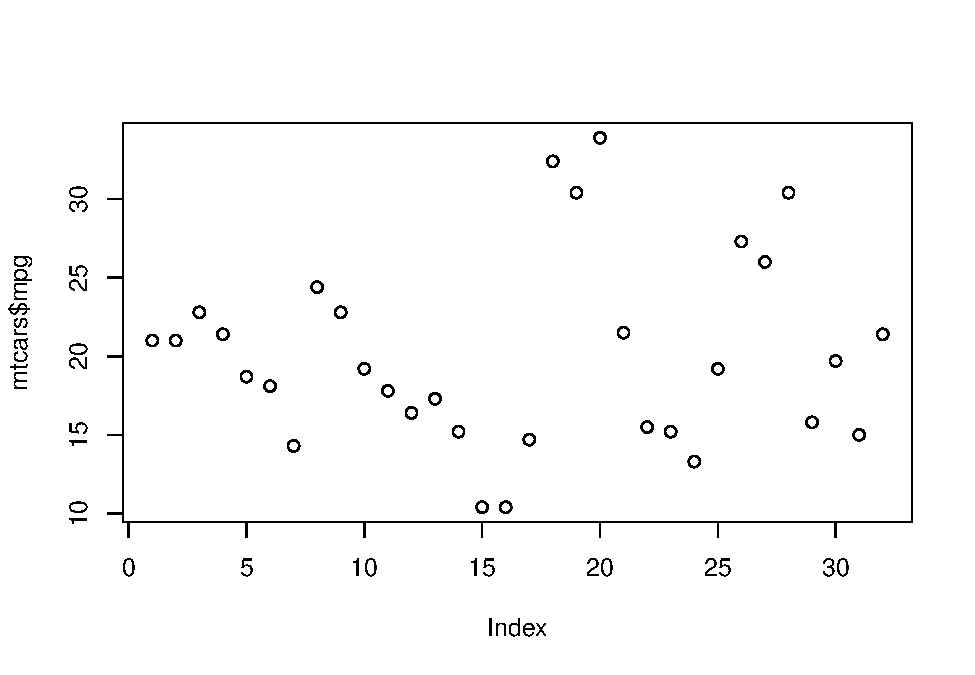
\includegraphics{210431461_CSC8639_Dissertation_files/figure-latex/fig2-1.pdf}
\caption{Another sample figure}
\end{figure}

You can use \textbf{bookdown} to allow references for Tables and
Figures.

\hypertarget{tables}{%
\subsection{Tables}\label{tables}}

Below we can see how to use tables.

See awesome Table\textasciitilde{}\ref{tab:table} which is written
directly in LaTeX in source Rmd file.

\begin{table}
 \caption{Sample table title}
  \centering
  \begin{tabular}{lll}
    \toprule
    \multicolumn{2}{c}{Part}                   \\
    \cmidrule(r){1-2}
    Name     & Description     & Size ($\mu$m) \\
    \midrule
    Dendrite & Input terminal  & $\sim$100     \\
    Axon     & Output terminal & $\sim$10      \\
    Soma     & Cell body       & up to $10^6$  \\
    \bottomrule
  \end{tabular}
  \label{tab:table}
\end{table}

You can also use R code for that.

\begin{Shaded}
\begin{Highlighting}[]
\NormalTok{knitr}\SpecialCharTok{::}\FunctionTok{kable}\NormalTok{(}\FunctionTok{head}\NormalTok{(mtcars), }\AttributeTok{caption =} \StringTok{"Head of mtcars table"}\NormalTok{)}
\end{Highlighting}
\end{Shaded}

\begin{longtable}[]{@{}lrrrrrrrrrrr@{}}
\caption{Head of mtcars table}\tabularnewline
\toprule
& mpg & cyl & disp & hp & drat & wt & qsec & vs & am & gear & carb \\
\midrule
\endfirsthead
\toprule
& mpg & cyl & disp & hp & drat & wt & qsec & vs & am & gear & carb \\
\midrule
\endhead
Mazda RX4 & 21.0 & 6 & 160 & 110 & 3.90 & 2.620 & 16.46 & 0 & 1 & 4 &
4 \\
Mazda RX4 Wag & 21.0 & 6 & 160 & 110 & 3.90 & 2.875 & 17.02 & 0 & 1 & 4
& 4 \\
Datsun 710 & 22.8 & 4 & 108 & 93 & 3.85 & 2.320 & 18.61 & 1 & 1 & 4 &
1 \\
Hornet 4 Drive & 21.4 & 6 & 258 & 110 & 3.08 & 3.215 & 19.44 & 1 & 0 & 3
& 1 \\
Hornet Sportabout & 18.7 & 8 & 360 & 175 & 3.15 & 3.440 & 17.02 & 0 & 0
& 3 & 2 \\
Valiant & 18.1 & 6 & 225 & 105 & 2.76 & 3.460 & 20.22 & 1 & 0 & 3 & 1 \\
\bottomrule
\end{longtable}

\hypertarget{lists}{%
\subsection{Lists}\label{lists}}

\begin{itemize}
\tightlist
\item
  Item 1
\item
  Item 2
\item
  Item 3
\end{itemize}

\hypertarget{refs}{}
\begin{CSLReferences}{0}{0}
\leavevmode\vadjust pre{\hypertarget{ref-data2017}{}}%
\CSLLeftMargin{{[}1{]} }
\CSLRightInline{Cabinet Office and Government Digital Service,
{``Government transformation strategy: Better use of data.''} HM
Government;
\url{https://www.gov.uk/government/publications/government-transformation-strategy-2017-to-2020/government-transformation-strategy-better-use-of-data},
2017.}

\leavevmode\vadjust pre{\hypertarget{ref-data2020}{}}%
\CSLLeftMargin{{[}2{]} }
\CSLRightInline{Department for Digital, Culture, Media \& Sport and
Department for Science, Innovation \& Technology, {``National data
strategy.''} HM Government;
\url{https://www.gov.uk/government/publications/uk-national-data-strategy/national-data-strategy},
2020.}

\leavevmode\vadjust pre{\hypertarget{ref-data2021}{}}%
\CSLLeftMargin{{[}3{]} }
\CSLRightInline{M. of Defence, {``Data strategy for defence,''}
\emph{GOV.UK}. HM Government;
\url{https://www.gov.uk/government/publications/data-strategy-for-defence/data-strategy-for-defence},
2021.}

\leavevmode\vadjust pre{\hypertarget{ref-data2022}{}}%
\CSLLeftMargin{{[}4{]} }
\CSLRightInline{Central Digital \& Data Office, {``Transforming for a
digital future: 2022 to 2025 roadmap for digital and data.''} HM
Government;
\url{https://www.gov.uk/government/publications/roadmap-for-digital-and-data-2022-to-2025/transforming-for-a-digital-future-2022-to-2025-roadmap-for-digital-and-data},
2022.}

\leavevmode\vadjust pre{\hypertarget{ref-trust}{}}%
\CSLLeftMargin{{[}5{]} }
\CSLRightInline{Centre for Data Ethics \& Innovation, {``Addressing
trust in public sector data use.''}
\url{https://www.gov.uk/government/publications/cdei-publishes-its-first-report-on-public-sector-data-sharing/addressing-trust-in-public-sector-data-use\#introduction--context}.}

\leavevmode\vadjust pre{\hypertarget{ref-pathway}{}}%
\CSLLeftMargin{{[}6{]} }
\CSLRightInline{Government Analysis Function, {``Types of data in
government learning pathway.''}
\url{https://analysisfunction.civilservice.gov.uk/learning-development/learning-pathways/types-of-data-in-government-learning-pathway/},
2022.}

\leavevmode\vadjust pre{\hypertarget{ref-onstool}{}}%
\CSLLeftMargin{{[}7{]} }
\CSLRightInline{Office for National Statistics, {``Time series
explorer.''}
\url{https://www.ons.gov.uk/timeseriestool?query=\&topic=\&updated=\&fromDateDay=\&fromDateMonth=\&fromDateYear=\&toDateDay=\&toDateMonth=\&toDateYear=\&size=50},
Unknown.}

\leavevmode\vadjust pre{\hypertarget{ref-datapoint}{}}%
\CSLLeftMargin{{[}8{]} }
\CSLRightInline{J. Donckt, J. Donckt, M. Rademaker, and S. Hoecke,
{``Data point selection for line chart visualization: Methodological
assessment and evidence-based guidelines.''} 2023. doi:
\href{https://doi.org/10.48550/arXiv.2304.00900}{10.48550/arXiv.2304.00900}.}

\leavevmode\vadjust pre{\hypertarget{ref-TVStore}{}}%
\CSLLeftMargin{{[}9{]} }
\CSLRightInline{Y. An, Y. Su, Y. Zhu, and J. Wang, {``TVStore:
Automatically bounding time series storage via time-varying
compression,''} in \emph{Proceedings of the 20th USENIX conference on
file and storage technologies}, in USENIX conference on file and STorage
technologies. Santa Clara, CA, USA: USENIX Association, 2022, pp.
83--99.}

\leavevmode\vadjust pre{\hypertarget{ref-Sveinn}{}}%
\CSLLeftMargin{{[}10{]} }
\CSLRightInline{S. Steinarsson, {``Downsampling time series for visual
representation.''} University of Iceland, Faculty of Industrial
Engineering, Mechanical Engineering; Computer Science, School of
Engineering; Natural Sciences, University of Iceland, Reykjavik,
Iceland, 2013.}

\leavevmode\vadjust pre{\hypertarget{ref-Shift}{}}%
\CSLLeftMargin{{[}11{]} }
\CSLRightInline{The Shift Project, {``Implementing digital
sufficiency,''} 2020.}

\leavevmode\vadjust pre{\hypertarget{ref-downsampling}{}}%
\CSLLeftMargin{{[}12{]} }
\CSLRightInline{W. Aigner, S. Miksch, W. Muller, H. Schumann, and C.
Tominski, {``Visual methods for analyzing time-oriented data,''}
\emph{IEEE Transactions on Visualization and Computer Graphics}, vol.
14, no. 1, pp. 47--60, 2008, doi:
\href{https://doi.org/10.1109/TVCG.2007.70415}{10.1109/TVCG.2007.70415}.}

\leavevmode\vadjust pre{\hypertarget{ref-sampling}{}}%
\CSLLeftMargin{{[}13{]} }
\CSLRightInline{B. C. Kwon, J. Verma, P. J. Haas, and C. Demiralp,
{``Sampling for scalable visual analytics,''} \emph{IEEE Computer
Graphics and Applications}, vol. 37, no. 1, pp. 100--108, 2017, doi:
\href{https://doi.org/10.1109/MCG.2017.6}{10.1109/MCG.2017.6}.}

\leavevmode\vadjust pre{\hypertarget{ref-MinMaxLTTB}{}}%
\CSLLeftMargin{{[}14{]} }
\CSLRightInline{J. Donckt, J. Donckt, M. Rademaker, and S. Hoecke,
{``MinMaxLTTB: Leveraging MinMax-preselection to scale LTTB.''} 2023.
Available: \url{https://arxiv.org/abs/2305.00332}}

\leavevmode\vadjust pre{\hypertarget{ref-transparency_obfuscation}{}}%
\CSLLeftMargin{{[}15{]} }
\CSLRightInline{N. A. Draper and J. Turow, {``The corporate cultivation
of digital resignation,''} \emph{New Media \& Society}, vol. 21, no. 8,
pp. 1824--1839, 2019, doi:
\href{https://doi.org/10.1177/1461444819833331}{10.1177/1461444819833331}.}

\leavevmode\vadjust pre{\hypertarget{ref-transparency_lack}{}}%
\CSLLeftMargin{{[}16{]} }
\CSLRightInline{M. Ananny and K. Crawford, {``Seeing without knowing:
Limitations of the transparency ideal and its application to algorithmic
accountability,''} \emph{New Media \& Society}, vol. 20, no. 3, pp.
973--989, 2018, doi:
\href{https://doi.org/10.1177/1461444816676645}{10.1177/1461444816676645}.}

\leavevmode\vadjust pre{\hypertarget{ref-social_transparency}{}}%
\CSLLeftMargin{{[}17{]} }
\CSLRightInline{J. Bates, H. Kennedy, I. Medina Perea, S. Oman, and L.
Pinney, {``Socially meaningful transparency in data-based systems:
Reflections and proposals from practice,''} \emph{Journal of
Documentation}, vol. ahead--of--print, 2023, doi:
\href{https://doi.org/10.1108/JD-01-2023-0006}{10.1108/JD-01-2023-0006}.}

\leavevmode\vadjust pre{\hypertarget{ref-transparency_fallacy}{}}%
\CSLLeftMargin{{[}18{]} }
\CSLRightInline{J. A. Obar, {``Sunlight alone is not a disinfectant:
Consent and the futility of opening big data black boxes (without
assistance),''} \emph{Big Data \& Society}, vol. 7, no. 1, 2020, doi:
\href{https://doi.org/10.1177/2053951720935615}{10.1177/2053951720935615}.}

\leavevmode\vadjust pre{\hypertarget{ref-political_transparency}{}}%
\CSLLeftMargin{{[}19{]} }
\CSLRightInline{K. E. Levy and D. M. Johns, {``When open data is a
trojan horse: The weaponization of transparency in science and
governance,''} \emph{Big Data \& Society}, vol. 3, no. 1, 2016, doi:
\href{https://doi.org/10.1177/2053951715621568}{10.1177/2053951715621568}.}

\end{CSLReferences}

\bibliographystyle{unsrt}
\bibliography{references.bib}


\end{document}
